Combining neural networks (NN) with reinforcement learning (RL) has led to many recent advances \cite{SOP, PPO, SAC, TRPO, SPU}.
Since training NNs requires diverse datasets and collecting real world data is expensive, most RL successes are limited to scenarios where the data can be cheaply generated in a simulation.
On the other hand, offline data is essentially free for many applications and RL methods should use it whenever possible.
This is especially true because practical deployments of RL are bottle-necked by its poor sample efficiency.
This insight has motivated a flurry of recent works in Batch RL \cite{siegel2020keep,agarwal2019optimistic,kumar2019stabilizing,fujimoto2019off,chen2019bail}.
These works introduce specialized algorithms to stabilize training from offline datasets.
However, offline datasets are not necessarily diverse.
In this work, we investigate how the properties of a diverse dataset influence the policy search procedure.
By collecting diverse offline dataset, we hope the networks will generalize without further training to unseen tasks or provide good initialization that speeds up convergence when we perform further on-policy training.

To collect diverse datasets, it occurs to us that we should collect data from different tasks.
However, datasets collected from different tasks may have state-action distributions with large divergence.
Such dataset bias presents a unique challenge in robust task inference.
We provide a brief description of the problem setting, the challenge and our contributions below.
For ease of exposition, we refer to such datasets as having little overlap in their state-action visitation frequencies thereafter.

We tackle the Multi-task Batch RL problem.
We train a policy from multiple datasets, each generated by interaction with a different task.
We measure the performance of the trained policy on unseen tasks sampled from the same task distributions as the training tasks.
To perform well, the policy must first infer the identity of the unseen tasks from collected transitions and then take the appropriate actions to maximize returns.
To train the policy to infer the task identity, we can train it to distinguish between the different training tasks when given transitions from the tasks as input.
These transitions are referred to as the context set \cite{rakelly2019efficient}.
Ideally, the policy should model the dependency of the task identity on both the rewards and the state-action pairs in the context set.
To achieve this, we can train a task identification network that maps the collected experiences, including both state-action pairs and rewards, to the task identity or some task embedding.
This approach, however, tends to fail in practice.
Since the training context sets do not overlap significantly in state-action visitation frequencies, it is possible that the learning procedure would minimize the loss function for task identification by \textit{only} correlating the state-action pairs and ignoring rewards, which would cause mistakes in identifying testing tasks.
This is an instance of the well-known phenomena of ML algorithms cheating when given the chance \cite{chu2017cyclegan} and is further illustrated in Fig. \ref{fig:cheat}.
We limit our explanations to the cases where the tasks differ in reward functions. Extending our approach to task distribution with different transition functions is easily done. We provide experimental results for both cases.

Our contributions are as follows.
To the best of our knowledge, we are the first to highlight the issue of the task inference module learning the wrong correlation from biased dataset.
We propose a novel application of the triplet loss to robustify task inference.
To mine hard negative examples, we approximate the reward function of each task and relabel the rewards in the transitions from the other tasks.
When we train the policy to differentiate between the original and relabelled transitions, we force it to consider the rewards since their state-action pairs are the same.
Training with the triplet loss generalizes better to unseen tasks compared to alternatives.
When we allow further training on the unseen tasks, using the policy trained from the offline datasets as initialization significantly increase convergence speed (up to $80\%$ improvement in sample efficiency).

To the best of our knowledge, the most relevant related work is \cite{siegel2020keep}, which is solving a different problem from ours.
They assume access to the ground truth task identity and reward function of the testing task.
Our policy does not know the testing task's identity and must infer it through collected trajectories.
We also do not have access to the reward function of the testing tasks.

% \begin{figure}[t]
%     \centering
%     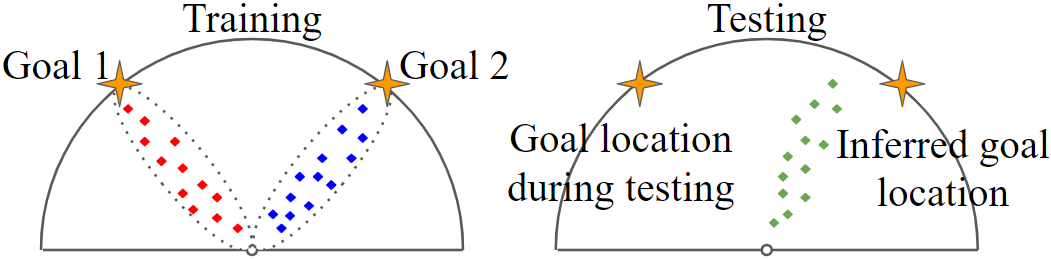
\includegraphics[width=0.7\textwidth]{chapter_2/fig/mismatch.png}
%     \caption{A toy example to illustrate the challenge. The agent must navigate from the origin to a goal location. \textbf{Left:} Goal 1 and Goal 2 denote the two training tasks. The red and blue squares indicate the transitions collected from task 1 and 2 respectively. We can train the task inference module to infer the task identity to be 1 when the context set contains the red transitions and 2 when the context set contains the blue transitions. Since there are no overlap between the red and blue squares, the task inference module learns to correlate the state-action pairs to the task identity. \textbf{Right:} The failure of the task inference module. The policy must infer the task identity from the randomly collected transitions, denoted by the green squares.
%         The agent needs to navigate to goal 1 during testing. However, if the green squares have more overlap with the blue squares, the task inference module will predict 2 to be the task identity. The agent therefore navigates to the wrong goal location.}
%     \label{fig:cheat}
% \end{figure}
